\subsection {Plug N' Play Database Wrappers}

The Erlang NetInf NRS includes functionality to allow for run-time database switching as well as providing an easy way to add interfaces to existing databases. Currently support for Riak is added, as well as a default Erlang list 'database' implementation. The database interface is designed to be very intuitive to implement. Figure \ref{fig:dbfig} shows the interface.

\begin{figure}[h!]
	\centering
\centerline{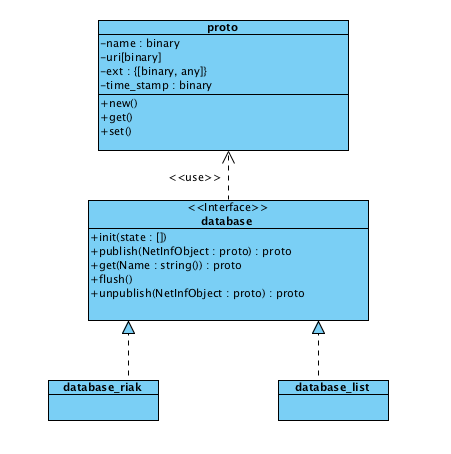
\includegraphics{./img/database_api.png}}
\caption{Database Interface}
\label{fig:dbfig}
\end{figure}

\subsection {Setup of Database Module}

All modules which wish to implement a database connection will use the custom nn\_database behaviour.

\begin {verbatim}
    -module(nn_database).
\end{verbatim}

The following functions must be implemented by all database wrappers

\textbf{Initialization}

\begin {verbatim}
    init() -> 
    	{ok, pid()} | {ok, registered_name:atom()} | {error, string()}
\end{verbatim}

The above function returns the connection for the specified database.
Remember the init should return an identifier to the persistent process of the specified database.

\begin {verbatim}
    publish(NetInfObject::nn_proto:proto()) -> 
    	{ok, ReturnNetInfObj::nn_proto:proto()}
\end{verbatim}

Takes the NetInfObject and returns: \{ok, NewObject\} where NewObject is the NDO created when merging the object being published with an object with the same name in the database. If there was no object with that name in the database, NewObject is the object being published.

\textbf{Get}

\begin {verbatim}
    get(Name::string()) -> 
    	{ok, nn_proto:proto()} | {ok, no_match}
\end{verbatim}

Takes the NetInf Name of the object and returns: \{ok, Data\} where Data is the NDO that was found or no\_match if not found.

\textbf{Unpublish}

\begin {verbatim}
    unpublish(NetInfObject::nn_proto:proto()) -> 
    	{ok, ReturnNetInfObj::nn_proto:proto()} | {ok, no_match}
\end{verbatim}

Takes the NetInfObject and returns \{ok, ReturnNetInfObj\} where ReturnNetInfObj is the NDO entry that was deleted from the specified database.

\textbf{Search}

\begin {verbatim}
    search(SearchList::list()) -> 
    	{ok, list()} | {ok, no_match}
\end{verbatim}

Takes a Erlang list of search keywords and returns a list of the NDO's which match those key words.

\textbf{Flush}

\begin{verbatim}
flush() -> ok
\end{verbatim}

Deletes all the entries in the database.   

Please see the module src/nn\_database\_list as an example of the wrapper implementation for use with a 'list' database in the source code.
